% *******************************************************************************
% * Copyright (c) 2007 by Elexis
% * All rights reserved. This document and the accompanying materials
% * are made available under the terms of the Eclipse Public License v1.0
% * which accompanies this distribution, and is available at
% * http://www.eclipse.org/legal/epl-v10.html
% *
% * Contributors:
% *    G. Weirich
% *
% *  $Id: vollversion.tex 2707 2007-07-06 11:03:07Z rgw_ch $
% *******************************************************************************
% !Mode:: "TeX:UTF-8" (encoding info for WinEdt)

\label{vollversion}
\index{Vollversion}
Bei Elexis müssen Sie eigentlich nichts weiter tun, um die Vollversion zu
erhalten, wenn Ihnen die Demo gefallen hat: Die Demo-Version \textbf{ist} die
Vollversion. Der einzige Unterschied ist die Datenbank.

Um Die Demo in eine Vollversion umzuwandeln, sind folgende Schritte nötig:
\begin{itemize}
  \item \glqq Echte\grqq{}Datenbank-Engine installieren. (\ref{dbengine})
  \item Die Demo-Datenbank löschen.
  \item Elexis mit dieser Datenbank-Engine verbinden (\ref{connect})
  \item Aktuelle Versionen der Stammdaten einlesen
  \item Elexis-Grundkonfiguration für Ihre Praxis erstellen
\end{itemize}
Allerdings sind diese Schritte nicht ganz trivial. Das Aktualisieren des
Datenbestands und vor allem das Erstellen einer korrekten Grundkonfiguration für
Ihre Praxis kann recht aufwändig sein. Hier kann sich Elexis nicht von anderen
Praxisprogrammen unterscheiden, da die Komplexität der Aufgabe für alle dieselbe
ist.
Wenn Sie dies selber machen wollen, sollten Sie sich genügend Zeit nehmen (einen
ganzen Tag), und dieses Kapitel exakt durchgehen. Wenn Sie nicht sicher sind,
empfehlen wir Ihnen, die Installation und Basiskonfiguration, zusammen mt einer
Instruktionsstunde für Ihr Praxispersonal einzukaufen.\par
Diese Anleitung ist zwangsläufig etwas schweizlastig. Für andere Länder sind vermutlich nicht alle Angaben korrekt bzw. brauchbar.
\bigskip

Der Vollständigkeit halber möchten wir noch darauf hinweisen, dass diese Dokumentation möglicherweise Fehler enthalten bzw. unvollständig sein könnte. Wir können keine Haftung dafür übernehmen, wenn Ihnen aus fehlerhafter Konfiguration oder wegen unkorrekter Dokumentation materielle oder immaterielle Schäden entstehen. Wir empfehlen Ihnen, alles sehr sorgfältig zu testen und wo möglich (z.B. Rechnungsstellung) auch manuell nachzukontrollieren, bevor Sie mit Ihrer Konfiguration \glqq echt\grqq{} arbeiten.
\section{Was Sie benötigen}
Bevor Sie mit der Konfiguration beginnen, sollten Sie die folgenden Programme und Daten zusammenstellen:
\begin{itemize}
  \item Ein Installationspaket für Ihren Datenbankserver
  \item Namen, Benutzernamen und Passwörter für alle, die Elexis benutzen sollen
  \item Namen, ZSR-Nummern, EAN-Nummern, Bankverbindungen bzw. Postcheckkonto, ESR-Teilnehmernummern von allen Mandanten
  \item Eine Aufstellung der bei Ihnen gültigen Taxpunktwerte
  \item Eine Vorstellung, wie Ihr Briefkopf auf Briefen, Rezepten, AUF-Zeugnissen aussehen soll
  \item Eine Liste der in Ihrem Praxislabor durchgeführten Untersuchungen, eingeteilt in Gruppen
  \item Medikamentenliste ICD-10, Tarmed, Analysenliste, MiGel, soweit benötigt 
  \item EAN-Nummern der Krankenkassen und Unfallversicherer
\end{itemize} 

\section{Datenbank-Engine installieren}
\label{dbengine}
Eine Elexis-Installation besteht aus zwei Teilen: Einem sogenannten \textit{Server}, auf dem die Daten 
abgelegt sind, und einem oder mehreren \textit{Clients}, welche auf die Daten zugreifen und diese darstellen
und bearbeiten lassen. Server und Client können auf ein- und demselben oder auf verschiedenen Computern sein.
Ein \textit{\textit{Server}} in einem weiteren Sinn ist ein eigener Computer, auf dem ein oder mehrere
Server-Programme laufen.

Als Server-Programm verwendet Elexis eine (im Prinzip beliebige) Datenbank, welche sich nach dem
Industriestandard JDBC bedienen lässt. Die automatische Einrichtung ist vorkonfiguriert für folgende
Datenbanksysteme:
\begin{itemize}
\item MySQL (\href{http://www.mysql.com}{www.mysql.com}): Dies ist die verbreitetste Datenbank im Internet. Die allermeisten
datenbank-basierten
 Web-Anwendungen verwenden einen MySQL-Server im Hintergrund. MySQL gilt als schnell, ausgereift und ist
 unkompliziert zu installieren. Für kommerzielle Zwecke kostet ein MySQL-Server ca. Fr. 750.-. Für private
 Zwecke ist er kostenlos.

\item PostgreSQL (\href{http://www.postgresql.org}{www.postgresql.org}): Dies ist
ein OpenSource Datenbankserver. Er beherrscht einen grösseren Befehlssatz als MySQL,
 gilt aber als etwas langsamer als dieser. Für unsere Zwecke sollte dies aber keine Rolle spielen, da die
 Geschwindigkeitstests sich üblicherweise im Bereich von einigen tausend Zugriffen pro Sekunde bewegen;
 ein Wert, der wohl nur in den wenigsten Arztpraxen erreicht werden dürfte. PostgreSQL ist kostenlos für alle
 Zwecke.

\item HSQLDB: Dies ist eine in Java geschriebene OpenSource-Datenbank. Sie kann sowohl als separater Server, als auch 
im Programm integriert verwendet werden. HSQL ist etwas langsamer, als die beiden erstgenannten Systeme, für kleinere 
Umgebungen aber eventuell genügend. Allerdings muss man ein besonderes Augenmerkt auf die Datensicherung legen, da ein 
Computerabsturz (oder versehentliches Ausschalten des PC, ohne das Programm herunterzufahren) die Datenbank unbrauchbar 
machen kann. HSQL ist kostenlos.
\end{itemize}

\textbf{Achtung}: Wir empfehlen den für die Demo verwendeten einfachen HSQL-Datenbankserver ausdrücklich \textit{nicht} für den Praxisgebrauch (Gefahr des Datenverlustes). Installieren Sie lieber MySQL oder PostgreSQL.
\begin{itemize}
 \item Wählen Sie am besten einen eigenen Computer als Server, an dem nicht direkt gearbeitet wird. Es dürfen aber ohne 
 weiteres mehrere Serverprogramme darauf laufen (z.B. Mailserver, Fax-Server, Druck-Server etc.).
 \item Installieren Sie dort den Datenbankserver Ihrer Wahl (Wir empfehlen mysql oder PostgeSQL)
 \item Erstellen Sie auf der Datenbank einen User-Account mit dem Namen elexisuser
 \item Erstellen Sie eine (leere) Datenbank mit dem Namen elexis, auf den 'elexisuser' Vollzugriff hat
 \item Entscheiden Sie sich unbedingt für eine Backupstrategie. Mehr Informationen dazu weiter unten.
 \item Die weitere Konfiguration erfolgt von den Clients aus. Der Server braucht im Alltagsbetrieb auch nicht unbedingt 
 Bildschirm und Tastatur, sondern er kann an irgendeiner kühlen Stelle der Praxis oder im Keller unauffällig 
 aufgestellt werden.
\end{itemize}

\textbf{Wichtig!}
\textit{Vergessen Sie nicht die Datensicherung!}

Elexis speichert sämtliche Daten in dieser Datenbank. Eine Zerstörung der Datenbank ist keineswegs unmöglich.
Ein Stromausfall kann die Festplatte  \glqq  auf dem linken Fuss\grqq{}  erwischen,
ein mechanischer Schaden kann wichtige Sektoren der Platte vernichten und sie
unlesbar machen, ein Fehler eines Programms kann die Daten löschen, ein Virus
kann sich an Ihren Daten austoben. Es gibt viele Datensicherungsstrategien, 
einige wollen wir hier vorstellen:

\begin{description}
\item[ Replikation ] Einige Datenbanken, wie z.B. MySQL ab Version 4.0 können ihre Daten laufend auf einen
auf einem anderen Computer laufenden Server kopieren. Da jeweils nur die geänderten Daten im Hintergrund
übertragen werden, kostet das weniger Leistung, als man vielleicht zunächst denken würde. Dieses Verfahren 
nennt man \textit{Replikation} . Im Endeffekt hat man dadurch zwei Datenbanken mit identischem Inhalt. 
Wenn der Server kaputt geht, kann man innert weniger Minuten den zweiten Rechner zum Server ernennen und
praktisch ohne Unterbruch weiterarbeiten.
\item [Virtual Machine] Ein verwandtes Konzept: Man lässt den Datenbankserver auf einer hierfür reservierten
 virtuellen Maschine laufen (z.b. von \href{http://www.vmware.com/}{VMWare}) und sichert in regelmässigen
 Abständen die komplette virtuelle Maschine. Bei einem Serverausfall kann man ebenfalls innert Minuten die
 Sicherungs-VM auf demselben oder irgendeinem anderen Computer im Netz starten und weiterarbeiten.
\item [Häufige Datensicherung] Man kann ein automatisiertes Backup alle paar Minuten durchführen
 (z.B. mit mysqldump), und die so gesicherten Daten in mehreren Generationen auf verschiedenen Datenträgern
 aufbewahren. Diese Methode braucht die wenigesten Ressourcen von den hier genannten und erzeugt die kleinsten
 Backup-Dateien. Dafür braucht man mehr Zeit, um bei einem Serverausfall weiterarbeiten zu können: Man muss
 zuerst den Datenbankserver auf einem Reservecomputer starten und dann dort die gesicherten Daten einspielen,
 anschliessend je nach Konfiguration alle Clients auf den neuen Server einstellen.
\end{description}

\section{Demo-Datenbank löschen}
Wenn Elexis beim Start eine Demo-Datenbank vorfindet, wird es immer mit dieser
verbinden,egal was Sie für Verbindungseinstellungen definiert haben. Sie müssen
deshalb jetzt Elexis beenden und dann die Demo-Datenbank löschen oder
umbenennen. Diese ist im Elexis-Programmverzeichnis im Verzeichnis \glqq
demoDB\grqq{} zu finden. Löschen Sie dieses Unterverzeichnis oder benennen Sie
es um. Danach können Sie Elexis wieder starten, es sollte sich jetzt mit Ihrer
vorher neu eingerichteten Datenbank verbinden können.

\section{Verbindung mit der Datenbank herstellen}
\label{connect}
Starten Sie Elexis und wählen Sie im Menu Datei -> Verbindung.

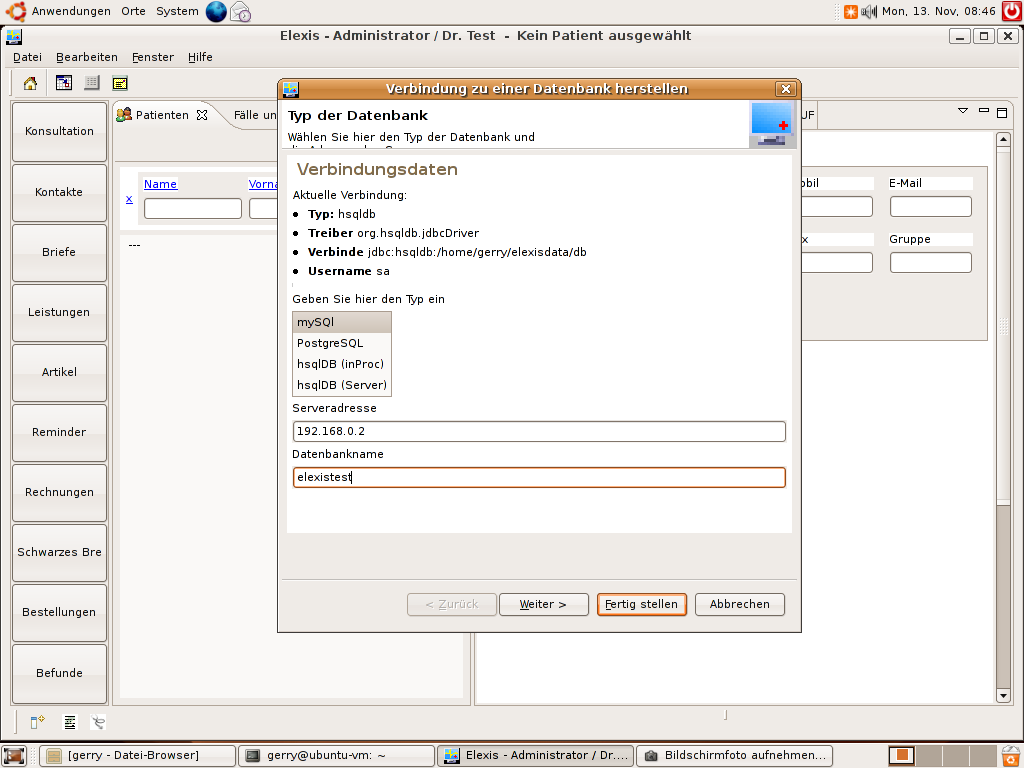
\includegraphics[width=0.9\textwidth]{images/verbindung11.png}
% verbindung11.png: 1024x768 pixel, 72dpi, 36.12x27.09 cm, bb=0 0 1024 768



Geben Sie den Typ der Datenbank (hier mysql), die Adresse des Servers (hier 192.168.0.2) oder dessen Internet-Namen 
(z.B. testserver.elexis.ch) ein, sowie den Namen der Datenbank (hier  elexistest) ein und klicken Sie auf 
\textit{weiter}.

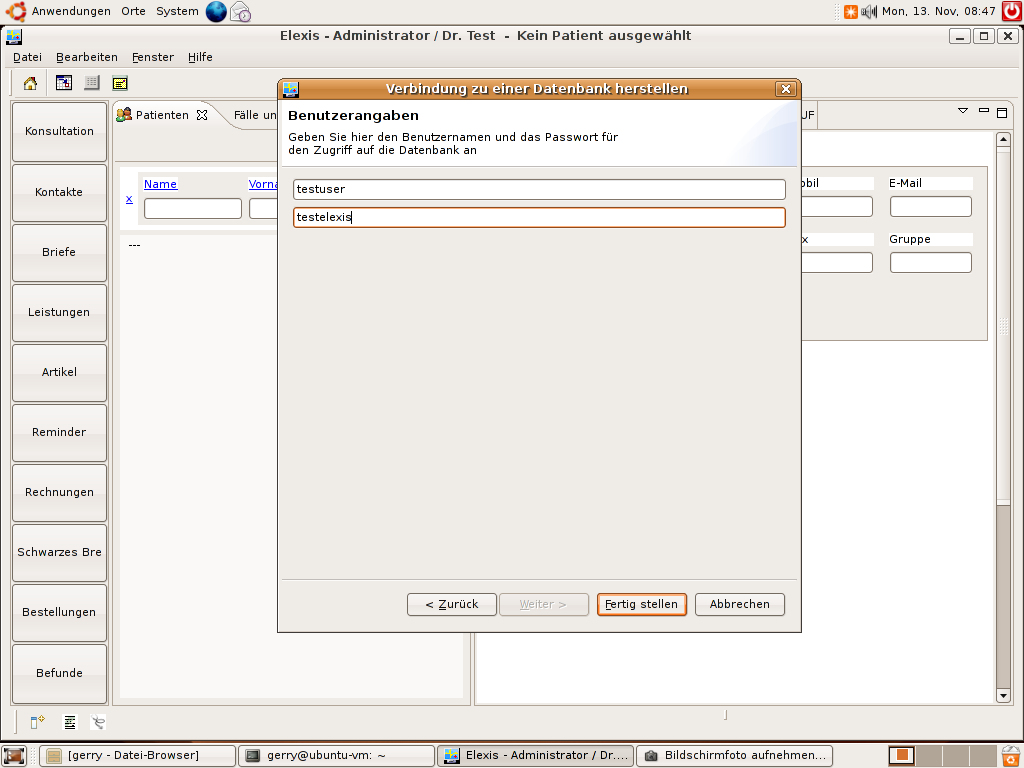
\includegraphics[width=0.9\textwidth]{images/verbindung12.png}
% verbindung12.png: 1024x768 pixel, 72dpi, 36.12x27.09 cm, bb=0 0 1024 768
Geben Sie hier in der oberen Zeile den Benutzernamen für die Datenbank (hier testuser) ein, in die untere Zeile das passende Passwort (hier testelexis) und klicken Sie auf \textit{fertig stellen}.

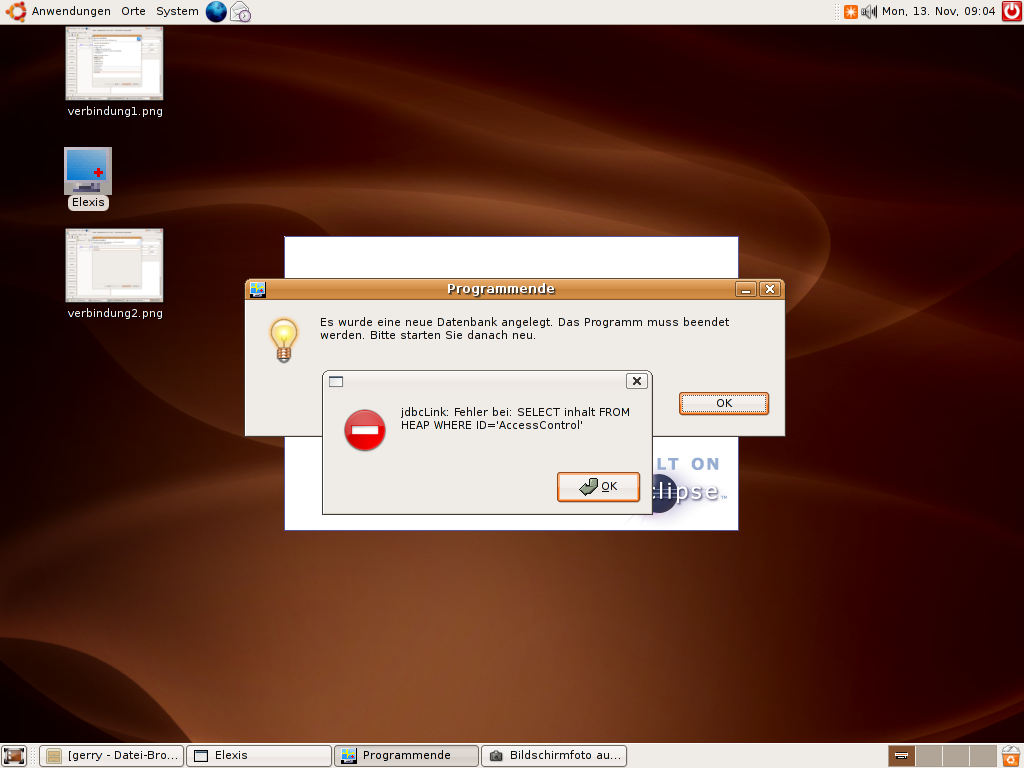
\includegraphics[width=0.9\textwidth]{images/verbindung13.png}
% verbindung13.png: 1024x768 pixel, 72dpi, 36.12x27.09 cm, bb=0 0 1024 768

 Es erscheinen einige Fehlermeldungen, die Sie wegklicken können. Danach müssen Sie das Programm nochmals neu starten.

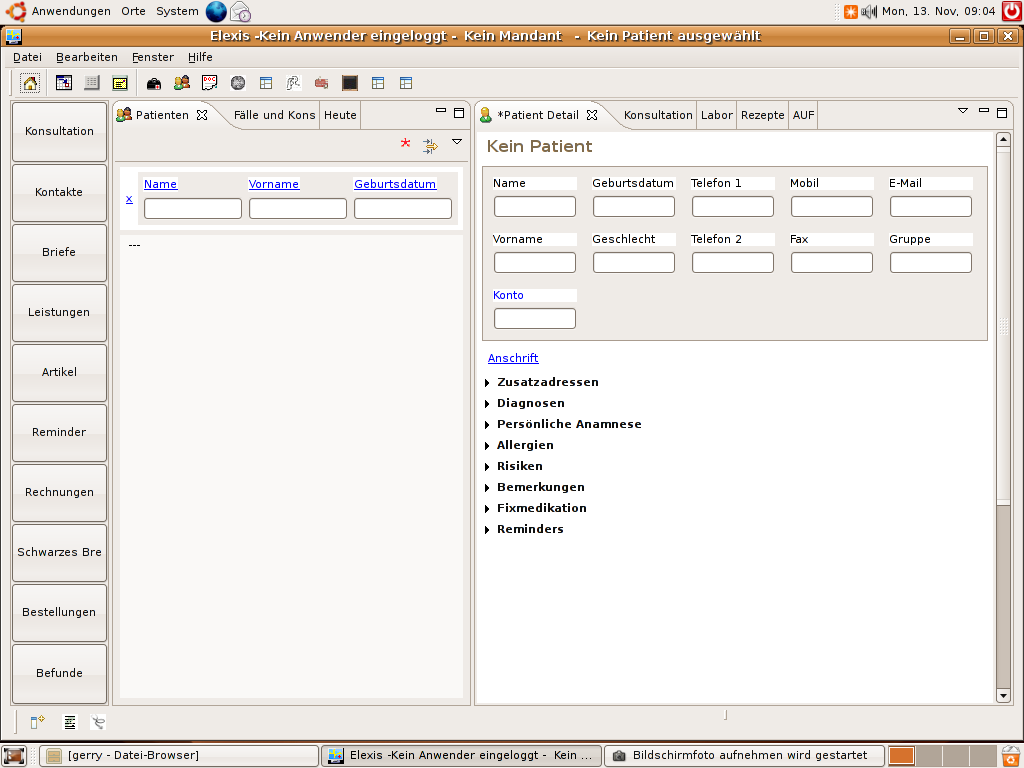
\includegraphics[width=4in]{images/verbindung14.png}
% verbindung14.png: 1024x768 pixel, 72dpi, 36.12x27.09 cm, bb=0 0 1024 768

Sie können sich jetzt mit dem Namen \textit{Administrator} und dem Passwort \textit{admin} an ihrem eben erstellten Elexis-System anmelden.

\section{Stammdaten einlesen}
\subsection{Tarmed}
\index{Tarmed}
Von www.tarmedsuisse.ch kann eine Microsoft-Access-Datenbank heruntergeladen werden. Binden Sie diese auf einem Windows-Computer als System-DSN ein. Gehen Sie in Elexis auf die Perspektive \textit{Codes}, wählen Sie dort den Reiter \textit{Tarmed} und rufen Sie das ViewMenu rechts auf. wählen Sie den Eintrag \textit{import} und geben Sie die eben konfigurierte Tarmed-DSN ein. Je nach Geschwindigkeit des PC wird der Import der gesamten Tarmed-Datenbank zwischen einer und 5 Minuten dauern. 
\subsection{ICD-10}
\index{ICD-10}
Von DIMDI können Sie den ICD-Katalog der WHO in computerlesbarer Form herunterladen. Sie benötigen die \textit{ICD-10-WHO-Systematik EDV-Fassung ASCII} und die \textit{ICD-10-WHO-2006 Systematik Metadaten ASCII}. Enpacken Sie beite Zip's ins selbe Verzeichnis. Die Warnung, dass eine Datei überschrieben wird, können Sie getrost ignorieren. Gehen Sie in Elexis auf die Codes-Perspektive und dort auf den Reiter \textit{ICD-10} und wählen Sie wieder \textit{import} aus dem View-Menu. Geben Sie in der folgenden Dialogbox das Verzeichnis an, in das Sie den ICD-Code entpackt haben.
\subsection{Medikamente und Medicals}
\index{Medikamente}\index{Medicals}\index{SL}
Diese beiden Gruppen werden aus derselben Datenbasis erstellt. Sie benötigen die Liste transfer.dat, die Sie z.B. vom www.e-mediat.ch im Abonnement beziehen können. Wählen Sie die Perspektive \textit{Codes}, dort den Reiter \textit{Medicals} bzw. \textit{Medikamente}, und dort wieder im View-Menu die Option Import und geben Sie dort die den Pfad zur Transfer.dat-Datei an.
\subsection{Analyseliste}
\index{Analysenliste}\index{AL}\index{EAL}
Diese wird vom BAG publiziert, allerdings leider aus unverständlichen Gründen nur in PDF-Form. Es ist deshalb ein zusätzlicher und potentiell fehlerträchtiger Konversionsschritt norwendig, um aus dieser PDF-Datei die Nutzdaten zu extrahieren. Sie benötigen dazu ein entsprechendes Programm, unter Windows beispielsweise TextFromPDF, unter Linux z.B. xpdf. Erstellen Sie mit diesem Hilfsprogramm eine plaintext-Version der Analysenliste, Gehen Sie in Elexis auf die Perspektive \textit{Codes} und dort auf den Reiter Analysen. Dort wieder den Import aus dem Viewmenu aufrufen und den Pfad der konvertierten Datei eingeben.
\subsection{MiGeL}
\index{MiGeL}
Auch die MiGeL-Liste wird vom BAG unverständlicherweise nur als PDF publiziert, die wir vor dem Import mühsam auseinandernehmen müssen. Sie benötigen erneut xpdf oder einen anderen PDF-nach-Text-Konverter und erstellen zunächst eine Textversion. Da die Struktur hier aber nicht so gut automatisch analysierbar ist, wie bei der Analysenliste, müssen Sie noch einen weiteren Schritt durchführen: Das Textfile muss in eine CSV-Tabelle umgewandelt werden, welche die Spalten code,text,einheit,preis enthält. Für diese Umwandlung können Sie beispielsewise OpenOffice Calc oder Microsoft Excel verwenden. Danach gehen Sie wiederum wie nun schon gewohnt auf die Perspektive \textit{codes}, dort auf den Reiter \textit{MiGel} und wählen dort \textit{import} aus dem VGiew-Menu.

\section{Grundkonfiguration}
\index{Grundkonfiguration}
\label{grundkonfiguration}
Die Grundkonfiguration umfasst folgende Schritte:
\begin{itemize}
  \item Mandanten und Anwender einrichten
  \item Laborparameter definieren
  \item Textvorlagen erstellen
  \item Abrechnungsmodul einrichten
\end{itemize}
\subsection{Mandanten und Anwender einrichten}
Öffnen Sie die Perspektive \textit{Kontakte},

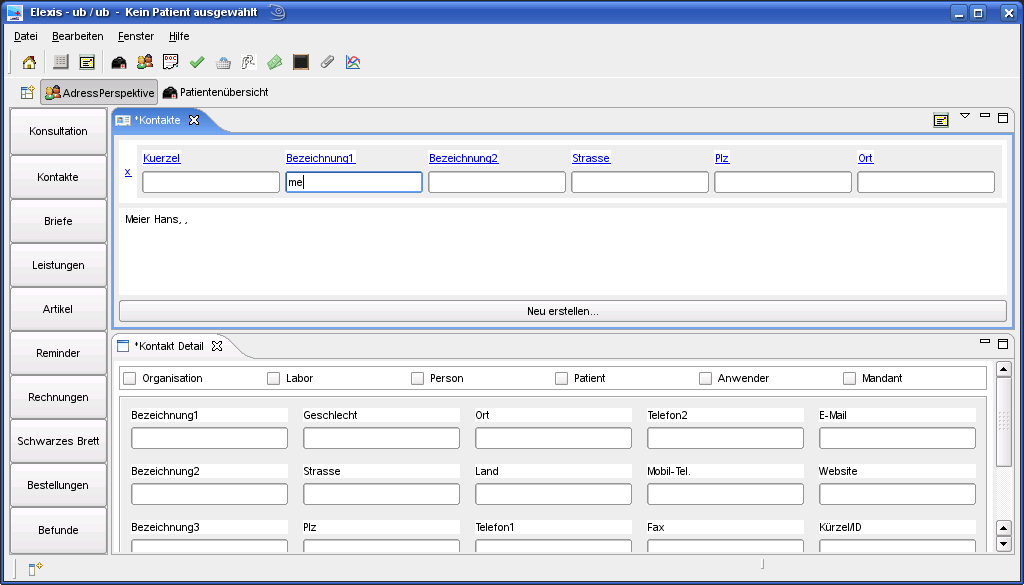
\includegraphics[width=4.5in]{images/grundkonfkonta.png}
% grundkonfkonta.png: 1024x585 pixel, 72dpi, 36.12x20.64 cm, bb=0 0 1024 585
\begin{itemize}
 \item Geben Sie unter \textit{Bezeichnung1} den Namen des neuen Mandanten oder Anwenders ein und klicken Sie auf \textit{Neu erstellen}
 \item Suchen Sie dann den eben erstellten Eintrag in der oberen Liste wieder auf, klicken Sie ihn an und ergänzen Sie die Angaben in der unteren Hälfte. Wie immer bei Elexis brauchen Sie nicht unbedingt alle Felder auszufüllen. \textit{Ernennen} Sie den eben erstellten Kontakt dann zum \textit{Mandanten} oder \textit{Anwender} (Ein Mandant ist immer auch gleichzeitig ein Anwender, und beide sind immer auch \textit{Personen}
 \item Wenn Sie alle Mandanten und Anwender so eingegeben haben, gehen Sie auf Datei-Einstellungen und dort auf den Reiter \textit{Zugriffsteuerung - Mandanten}
\end{itemize}

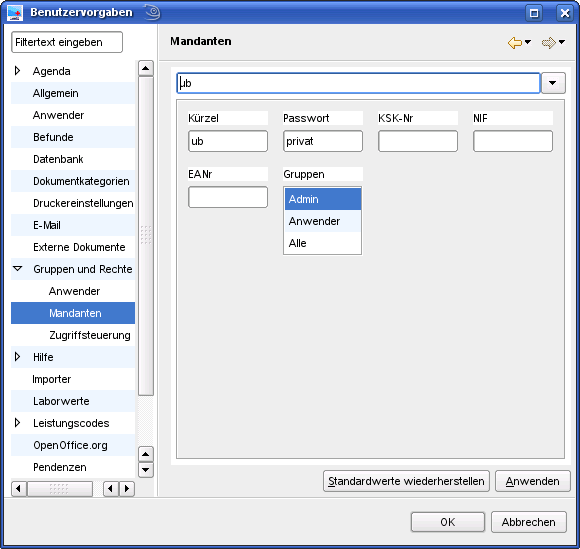
\includegraphics[width=4in]{images/grundkonfmand.png}
% grundkonfmand.png: 580x549 pixel, 72dpi, 20.46x19.37 cm, bb=0 0 580 549
\begin{itemize}
 \item Geben Sie dort die entsprechenden Angaben für Ihre eingerichteten Mandanten ein. Für \textit{Kürzel} muss der Anmeldename angegeben werden, für Passwort das Anmeldepasswort. Die restlichen Daten hängen vom Typ des Mandanten ab.
 \item Gehen Sie dann zum Abschnitt Zugriffsteuerung - Anwender
\end{itemize}

Geben sie dort für alle definierten \index{Anwender}Anwender die entsprechenden Daten ein. Vergessen Sie auch nicht, allen Anwendern einen existierenden Standard-Mandanten zuzuordnen (\textit{Für Mandant}). Auch für bereits angelegte Mandanten-Einträge (die Sie auch in der Anwender-Einstellung wiederfinden, da alle Mandanten auch Anwender sind), sollte ein Standard-Mandant festgelegt werden (Normalerweise er selbst). Der Zugeordnete Mandant definiert, in wessen Auftrag und auf wessen Rechnung der betreffende Anwender normalerweise arbeitet. Dies kann während der Arbeit geändert werden (Unter \textit{Datei - Mandant}...), aber beim Einloggen wird immer zunächst der Standard-Mandant eingestellt.

\subsection{Laborparameter eingeben}
Öffnen Sie zunächst wieder die \textit{Kontakte-View}. Geben Sie dort Ihr Eigenlabor und ihre externen Labors ein. Markieren Sie diese als \textit{Labor}

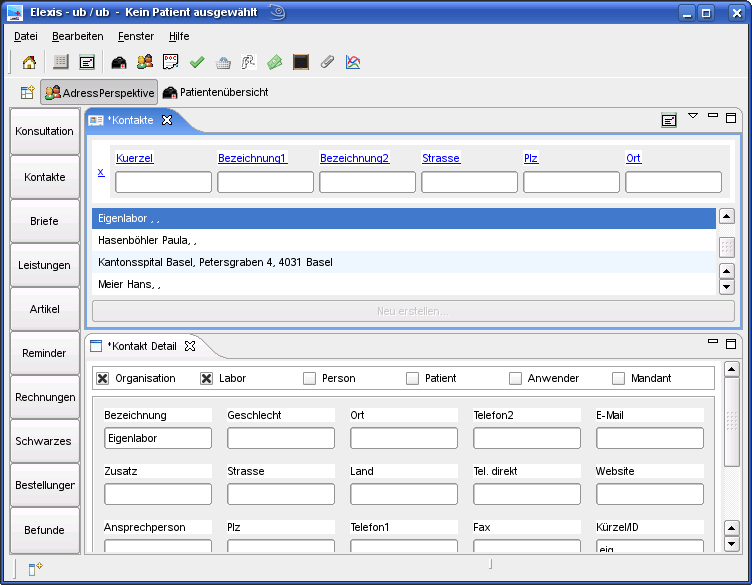
\includegraphics[width=4in]{images/grundkonfmand1.png}
% grundkonfmand1.png: 752x585 pixel, 72dpi, 26.53x20.64 cm, bb=0 0 752 585
\subsection{Textprogramm konfigurieren}

Elexis arbeitet bisher nur mit OpenOffice zusammen. Deshalb wird hier auch nur die Konfiguration mit OpenOffice erläutert.

\begin{itemize}
 \item Falls noch nicht geschehen: Installieren Sie OpenOffice (Mindestens Version 2.0)
 \item Wählen Sie in Elexis \textit{Datei-Einstellungen-Textverarbeitung}
\end{itemize}

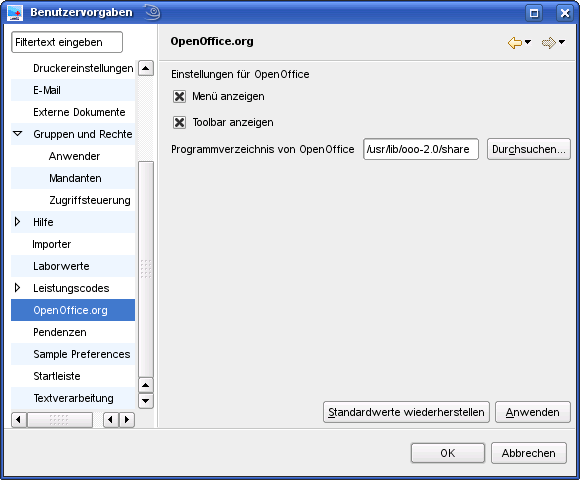
\includegraphics[width=3.5in]{images/grundkonfmand2.png}
% grundkonfmand2.png: 580x480 pixel, 72dpi, 20.46x16.93 cm, bb=0 0 580 480

\begin{itemize}
 \item Suchen Sie den Pfad des \textit{program} Unterverzeichnisses der OpenOffice Installation auf. Unter Windows wird das standardmässig in c:/programme/OpenOffice.org 2.0/program sein, bzw. an der Stelle, wo Sie OpenOffice installiert haben.
 \item Drücken Sie \textit{Apply}, Schliessen Sie die Konfiguration und starten Sie Elexis neu
 \item Wenn Sie jetzt z.B, die Briefe-Perspektive anwählen, sollte das Fenster von OpenOffice innerhalb des Elexis-Fensters erscheinen. (Dies wird beim ersten Mal recht lange dauern, d.h. ca. 30 Sekunden)
\end{itemize}

\subsubsection{\index{Vorlagen!Druckvorlagen}Druckvorlagen erstellen}
Für einige Formulare sucht Elexis nach vordefinierten Druckvorlagen mit einem festgelegten Namen. Diese definieren das für Ihre Anwendung spezifische Aussehen dieser Formulare. Es müssen jeweils Platzhalter für Variable Daten an den passenden Stellen eingefügt werden.

Um eine Formatvorlage zu erstellen, gehen Sie am besten so vor: Schreiben Sie die Vorlage ganz normal in der Textverarbeitung und speichern Sie sie als normales Textdokument. Von Elexis aus wählen Sie dann die Perspektive \textit{Briefe} und rufen das

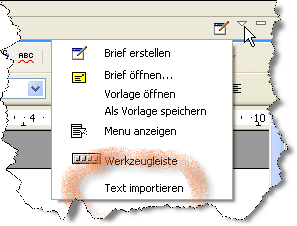
\includegraphics[width=2.5in]{images/import.png}
% import.png: 297x226 pixel, 96dpi, 7.86x5.98 cm, bb=0 0 223 169

ViewMenu rechts auf.

Wählen Sie dort \textit{Text importieren} und suchen Sie ihre vorher erstellte Vorlage auf.
 Hierdurch wird das Dokument nach Elexis importiert. Sie können jetzt noch Änderungen anbringen, rufen Sie dann wieder das ViewMenu rechts auf und wählen Sie diesmal \textit{Als Vorlage speichern}.

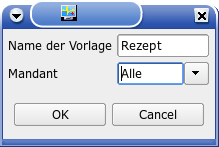
\includegraphics[width=2.5in]{images/rezept1.png}
% rezept1.png: 219x147 pixel, 72dpi, 7.73x5.19 cm, bb=0 0 219 147

Für \textit{Name der Vorlage} müssen Sie bei den unten aufgelisteten Standardvorlagen den entsprechenden Namen geben, für eigene Vorlagen können Sie beliebige Bezeichnungen einsetzen. Unter \textit{Mandant} können Sie einstellen, für welchen Mandanten diese Vorlage ist (oder ob für alle)

Im Folgenden jetzt eine Liste der erwarteten Standard-Vorlagen:

\begin{itemize}
\item Rezept: \index{Vorlagen!Rezept}Hierfür wird eine Formatvorlage mit dem Namen \textit{Rezept} benötigt. Diese kann z.B. so aussehen:
 \end{itemize}
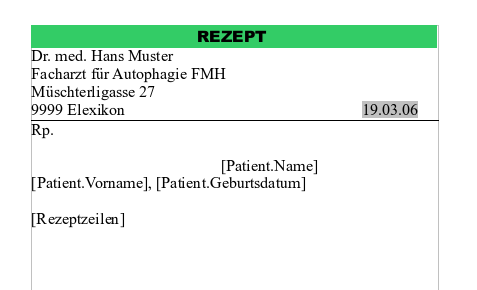
\includegraphics[width=4in]{images/rezept.png}
% rezept.png: 477x290 pixel, 72dpi, 16.83x10.23 cm, bb=0 0 477 290

An der Stelle, wo [Rezeptzeilen] steht, werden später die ausgewählten Medikamente eingesetzt. Dieser Platzhalter ist somit notwendig. Alle anderen Elemente der Vorlage \textit{Rezept} sind fakultativ.

\begin{itemize}
 \item \textit{AUF-Zeugnis}: Eine Formatvorlage für Arbeitszeugnisse. Als Platzhalter können [AUF.Grund], [AUF.von], [AUF.bis], [AUF.Prozent] und alle Standard-Platzhalter eingesetzt werden. Alle sind fakultativ.


 \item \textit{Laborblatt}: Für das Ausdrucken von Laborwerten. Die Laborwerte werden beim Platzhalter [Laborwerte] eingesetzt, dieser Platzhalter ist zwingend, andere können nach Wahl gesetzt werden.
 \item \textit{Liste}: Für das Audrucken veschiedener in Listenform vorliegender Daten. An einer Stelle muss ein Platzhalter [Liste] sein, an den dann die Daten eingefügt werden können.
\end{itemize}

Je nachdem können von Ihnen verwendete Plugins ebenfalls bestimmte Vorlagen benötigen

\subsection{Abrechnungsmodul einrichten}
\label{conf:abrechnung}
Diese Einrichtung muss unbedingt durchgeführt werden, bevor die ersten Leistungen verrechnet werden. Das genaue Vorgehen hängt vom Abrechnungsmodul ab. Für das Arztarif-Schweiz-Modul ist das Vorgehen bei der Besprechung des entsprechenden Plugins beschrieben. (S. \ref{arzttarife}, Seite \pageref{arzttarife} ff.)

